Dos masas cuelgan en serie de un soporte fijo: el resorte \(k_1\) une el soporte a \(m_1\)
y el resorte \(k_2\) une \(m_1\) a \(m_2\). Sean
\[m_1=1\ \mathrm{kg},\quad m_2=1.25\ \mathrm{kg},\quad k_1=k_2=100\ \mathrm{N/m}.\]
Determinar las frecuencias naturales de las pequeñas oscilaciones verticales sin amortiguamiento,
medidas desde el equilibrio estático.

\Needspace{8.14cm}
\begin{center}
\begin{minipage}{\linewidth}
\centering
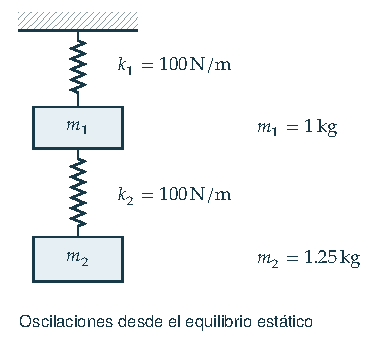
\includegraphics[width=7.21cm]{assets/M2-E0070-setup.pdf}\par
\smallskip{\small Conexión en serie de los dos muelles y las dos masas.\par}
\end{minipage}
\end{center}
